\documentclass[a4paper,11pt,oneside]{report}
\usepackage[pdftex]{graphicx}
\usepackage[utf8x]{inputenc}
\usepackage[spanish]{babel}
\usepackage{fancyhdr}
\usepackage[Bjornstrup]{fncychap}
\usepackage{tabularx}
\usepackage{hyperref}
\usepackage{eurosym}
% \usepackage[usenames,dvipsnames]{color}
% \usepackage{colortbl}
% \usepackage[caption=false]{subfig}
% \usepackage{float}
% \usepackage{pdflscape}

\setlength{\headheight}{25pt}
\setlength{\parskip}{6pt}

% Margenes 1cm mas pequennos
% \addtolength{\oddsidemargin}{-1cm}
% \addtolength{\evensidemargin}{-1cm}
% \addtolength{\textwidth}{2cm}
% \addtolength{\voffset}{-1cm}
% \addtolength{\textheight}{2cm}


\chead{}
\rhead{\nouppercase{\leftmark}}

\hypersetup{
colorlinks,
citecolor=black,
filecolor=black,
linkcolor=black,
urlcolor=black
}

 % La que hay que liar para que las cabeceras de los capitulos
 % no tiren media pagina a la basura...

\makeatletter
\def\@makechapterhead#1{{
\parindent \z@ \raggedright \normalfont
\ifnum \c@secnumdepth >\m@ne
	\if@mainmatter
		\DOCH
	\fi
\fi
\interlinepenalty\@M
\if@mainmatter
	\DOTI{#1}
\else
	\DOTIS{#1}
\fi
}}

\def\@makeschapterhead#1{{
\parindent \z@ \raggedright
\normalfont
\interlinepenalty\@M
\DOTIS{#1}
}}
\makeatother

\begin{document}


\pagestyle{plain}

%%%% Title Page %%%%%

\pagenumbering{alph}

\begin{titlepage}
\begin{center}

% Upper part of the page

\includegraphics[width=0.4\textwidth]{esi_bw.png}\\[1cm]
\textsc{\LARGE Escuela Superior de Informática}\\[0.5cm]
\textsc{\Large Universidad de Castilla -- La Mancha}\\[2.5cm]

% Title
{\LARGE Diseño y fabricación por computador}\\[0.5cm]
\rule{\linewidth}{0.5mm}\\[0.4cm]
{\huge \textbf{Material y análisis del producto}}\\[0.4cm]
\rule{\linewidth}{0.5mm}\\[1.5cm]


{\large
\begin{tabular}{l}
\hspace{1cm}\textbf{\emph{Autor}}\\
Antonio Gómez Poblete \\
\end{tabular}
% \end{minipage}
}
\vfill

% Bottom of the page
{\large \today}\\[0.5cm]

\end{center}
\end{titlepage}

%%%% end Title Page %%%%%

\clearpage
\pagenumbering{arabic}

\tableofcontents
\addcontentsline{toc}{chapter}{\contentsname}
% \listoffigures
% \listoftables

\clearpage

\pagestyle{fancy}

\chapter{Material}
\section {Definición}

	\subsection {Características físicas}

	\subsection {Características químicas}

	\subsection {Características mecánicas}

\section {Estracción/obtención}

	\subsection {Extracción/Síntesis}

	\subsection {Proceso de obtención}


\chapter{Producto}
\section {Descripción general del producto}
	El producto que se desea fabricar es una mesa de billar. En particular una mesa de \emph{pool}.
El producto esta formado por una  mesa con un tablero de pizarra forrada de paño, rodeada de bandas de material elástico y con seis troneras. 
	
	\subsection {Utilidad y aplicaciones}
	La mesa de billar es usada para la práctica de un deporte llamado billar. Este deporte olímpico desde el 2004, tubos sus inicios en la 
 antigua  Grecia y Egipto, pero es en la Europa del siglo XV cuando se empezó a tomar la forma del juego que se conoce en la actualidad. 

El billar consiste en: impulsar un número variable de bolas con la ayuda de un taco,  el cual lleva adosado en su extremo anterior una suela de cuero.
Con este movimiento debemos procurar introducir unas bolas (de materiales sintéticos con cualidades elásticas similares a las del marfil) dentro de las troneras.

	\subsection {Mercado}

El mercado de este productos suele abarcarlo en casi su totalidad los locales de ocio,(bares y recreativos...). También hay particulares que desean obtener una
mesa de billar, pero debido a su coste elevado son pocos los que pueden permitirse tener una en sus hogares. 
    
\section {Diseño del producto}

	\subsection {Definición técnica (dimensiones, especificaciones técnicas)}
			\begin{enumerate}
			\item Las mediadas de la mesa de billar pueden variar ligeramente siempre y cuando respetemos algunas medidas estándar. En este caso las medidas elegida para la mesa son:
				\begin{itemize}      
				\item Medidas del campo de juego del billar: 200 x100 cm.

				\item Medidas exteriores: 232 x 132 Altura: 80cm
				\end{itemize}
				

			\item La superficie de la mesa es una la losa de pizarra 20 mm. Recubierta de un fieltro(lana y poliamida) verde de 600g.

			\item Los bordes del campo de juego en los que las bollas tienen que rebotar esta compuesto por (goma vulcanizada + lana)
			\end{enumerate}


	\subsection {Definición geométrica}
		    \begin{enumerate}
		     \item La superficie del juego debe ser rectangular y poseer 6 agujeros por donde se introducirán las bollas de x cm. Lo  agujeros estarán distribuidos como
			    muestra la siguiente figura.
		     \item Los bordes del campo (goma) están por todo el perímetro del campo salvo por donde hay agujeros y mide  3 cm de grosor.

		     \item Para la definición geométrica de como son las demás piezas  se adjunta vistas que explique mejor que con palabras que apariencia tiene la mesas de billar
			  y sus diferentes elementos.
		\begin{center}
    			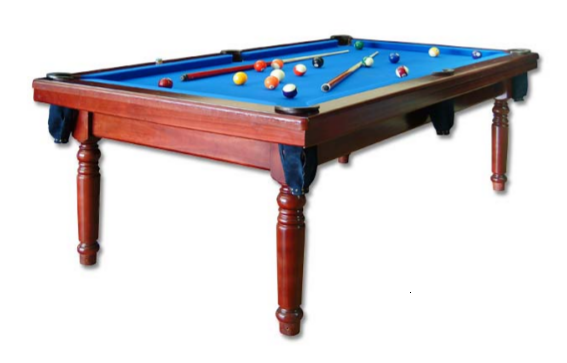
\includegraphics[width=0.8\textwidth]{donbillar.png}
		\end{center}	
		    \end{enumerate}


		    

	\subsection {Definición mecánica}
		    Cuando una bola cae a un agujero se pueden fabricar muchos y muy complejos mecanismos de recogida de la bola pero un mecanismo muy extendido,
		    fiable y muy empleado en las mesas de billar, que residen en las viviendas, es poner unas troneras que guarden la bola una vez caida por el agujero hasta que queramos empezar
		    el juego de nuevo. Estas troneras o recipientes pueden ser de muchos materiales pero en nutro caso serán de plástico duro y lo suficientemente grandes como para quepan casi todas las bolas. 
\section {Fabricación del producto}

	\subsection {Recepción de piezas y/o materiales}

	\subsection {Proceso de fabricación detallado}
		A  continuación vamos a  ir detallando paso por paso como se fabrica una mesa de billar y sus diferentes piezas.
		
		\subsubsection {Preparar el tablero de pizarra}
			En primer lugar vamos a explicar como fabricar la pieza base de la mesa, el tablero o superficie de juego, hecho de pizarra. Este no tiene que ser necesariamente de pizarra pero es el mejor material, debido a  su resistencia y elasticidad, y no todas las pizarras son igual de buenas para una mesa de billar, lo que hace que una pizarra se buena y otra no es el contenido en cuarzo, cuanto menos tenga mejor será.

Para poder llegar hasta la pizarra solo se puede hacer combinar potentes motosierras con dinamita para obtener bloque gigantescos de pizarra.

	\begin{center}
	    		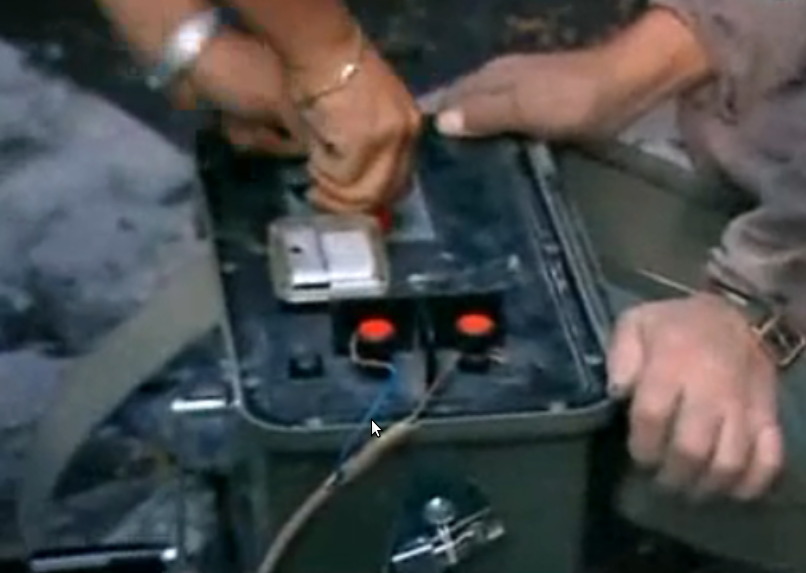
\includegraphics[width=0.4\textwidth]{Pantallazo-1.png}
			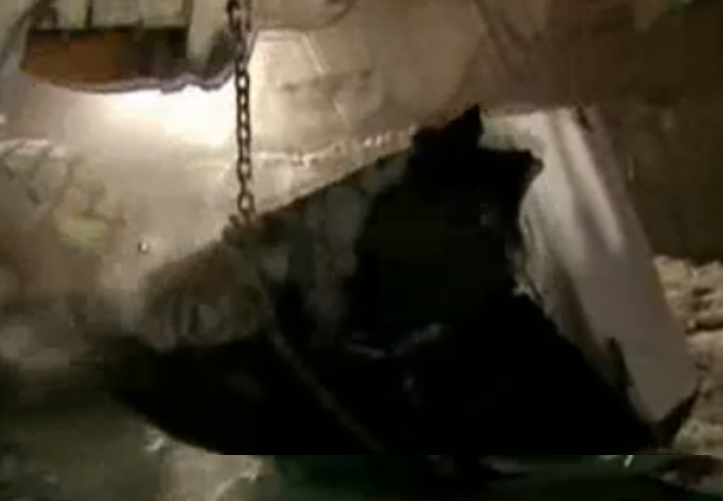
\includegraphics[width=0.4\textwidth]{Pantallazo-2.png}
	\end{center}

 Cuando tenemos el bloque de pizarra esté es trasportado a una marmolería donde se trasformara en la pieza que formará la mesa de billar.


Como el bloque de pizarra es enorme  no se pueda partir  en trozos que sirvan para una mesa de billar, primero hay que cortar el bloque en losas que se puedan manejar. Para ello se utiliza una enorme sierra que corta la pizarra en gruesas lonchas. Para evitar que la pizarra se quiebre hay que cortarla muy despacio y refrigerar con agua continuamente las hojas de las sierras. 
	\begin{center}
	    		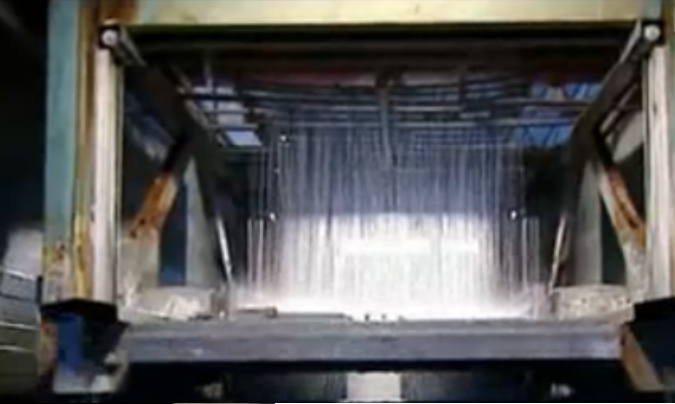
\includegraphics[width=0.4\textwidth]{Pantallazo-3.png}

	\end{center}


Como la pizarra esta formada por una serie de capas asentadas una sobre otra, los cortes tienen que ser hechos  a lo largo de esa linea de división.  La estructura rígida    
de la pizarra hace que si se corta en la dirección correcta producirá losas finas de un grosor uniforme, para ello se emplea un cincel y un martillo para separa las losas de pizarra de forma manual.
	\begin{center}
	    		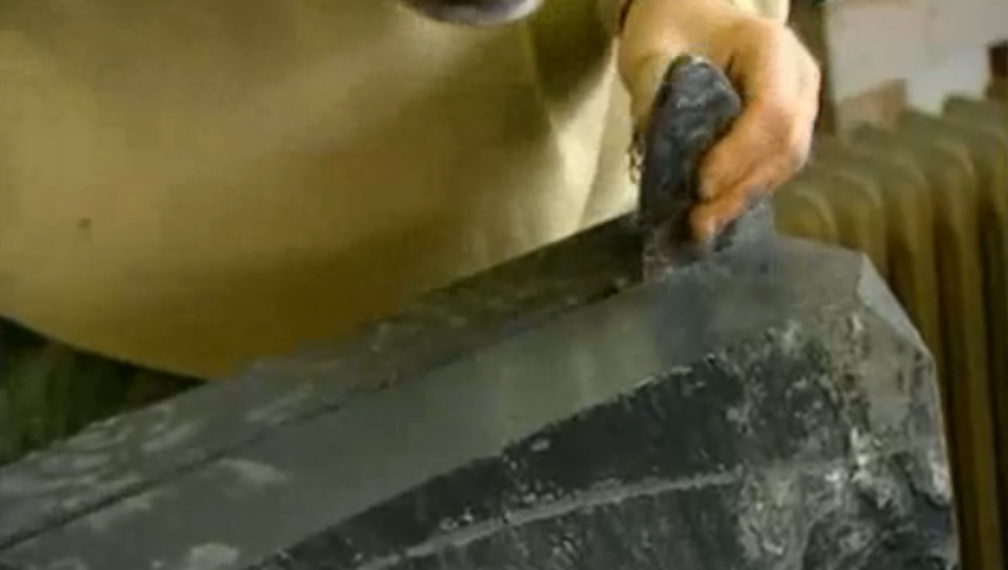
\includegraphics[width=0.4\textwidth]{Pantallazo-5.png}

	\end{center}

Cuando ya tenemos la losa de pizarra la cortamos con las dimensiones deseadas (2m x 1m) ayudándonos de unas radiales. 
\begin{center}
	    		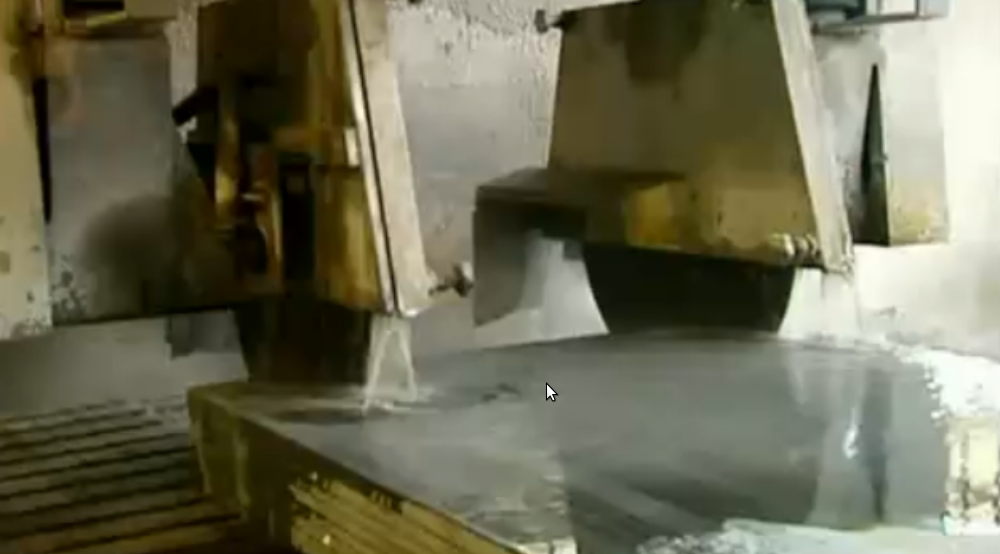
\includegraphics[width=0.4\textwidth]{Pantallazo-6.png}

	\end{center}

Luego hay que  pulir los bordes con ayuda una muela de diamante que los deje suaves y nivelados.

Una cuarta maquina corta los agujeros por donde salen las bolas para que luego sean ligados a mano.

\begin{center}
	    		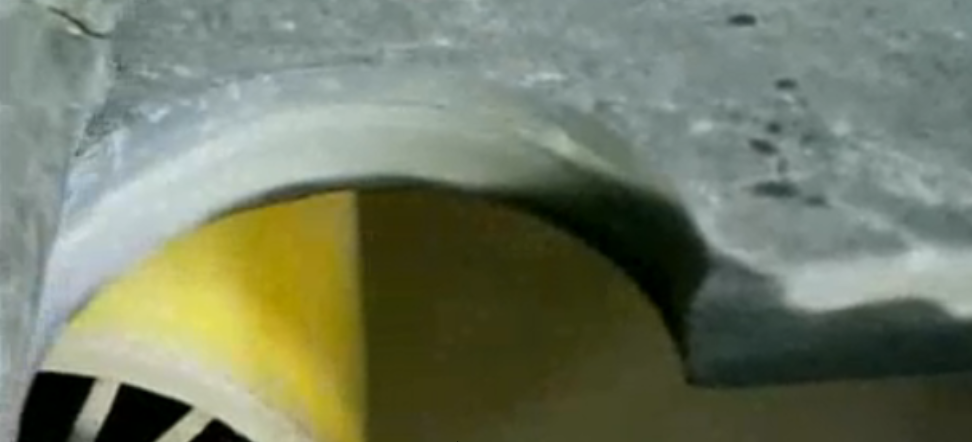
\includegraphics[width=0.4\textwidth]{Pantallazo-7.png}

	\end{center} Y con esto concluye la preparación del la losa de pizarra.
 
		\subsubsection {Colocación del paño}
  	
 	Para un perfecto deslizamiento de la bola sobre la losa de pizarra hay que colocar un paño de lana y poliamida azul en nuestro caso. Este deberá ser muy resistente y tener una superficie uniforme para desempeñas correctamente su función.

	La coloración del paño o tapiz se hace de forma totalmente artesanal. Para ello lo colocan primero encima de da losa y entre los agujeros por donde salen las bolas , luego cortan el paño sobrante y finalmente la alisan con un cepillo. 

	\begin{center}
    			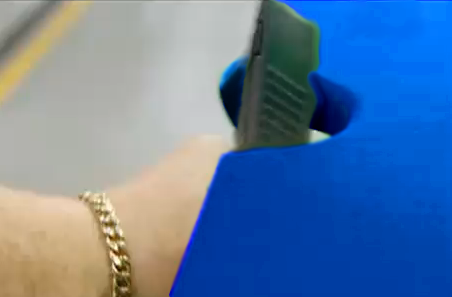
\includegraphics[width=0.4\textwidth]{Pantallazo.png}
		\end{center}
   
		\subsubsection { Montaje del  borde superior de la mesa de billar}

	En este paso se montara la parte de arriba de la mesa  sin incluir la superficie de juego.

	
	Los borde de la superficie de juego deben de tener la elasticidad correcta como para que las bolas reboten sin perder parte de su energía cinética, para ello se hace un compuesto de goma vulcanizada (proceso mediante el cual se calienta el caucho crudo en presencia de azufre, con el objetivo de incrementar su dureza y resistencia al frío).

Luego a los borde se les colocan también unos pliegues de tapetes azules de lana sujetos con unas grapas.


\section {Mercado}

	\subsection {Comercialización del producto}


\subsection{bibliografía}

%http://www.donbillar.com/mesas_de_billar.html

%http://www.youtube.com/watch?v=8cjHNDAokqs

%http://construyeloya.blogspot.com/2007/09/construye-tu-propia-mesa-de-billar.html

%http://www.construirmesadebillar.com/




\end{document}
